%%% -*- TeX-engine: xetex -*-
\documentclass{beamer}

% for themes, etc.
\usepackage{times}  % fonts are up to you
\usepackage{graphicx}
\usepackage{color}
\usepackage{hyperref}

\mode<presentation>
{
  \usetheme{Warsaw}
  \useoutertheme{infolines}
  \usecolortheme{whale}
  \setbeamertemplate{navigation symbols}{}
}
\usepackage{fontspec}
\usepackage{xunicode}
\usepackage[BoldFont,SlantFont]{xeCJK}
\setCJKmainfont{SimSun}
\setCJKmonofont{SimHei}

\title{
  基于翻译技术的流量调度研究 \\
  中期报告
}
\author{王文鑫}
\date{2016年4月15日}
% \AtBeginSection[]
% {
% \begin{frame}<beamer> 
%   \tableofcontents[currentsection]
% \end{frame}
% }

\begin{document}

\begin{frame}
  \titlepage
\end{frame}

\section{研究目标}

\begin{frame}
  \frametitle{研究目标}

  存在多种运营商IPv4出口时,二级翻译器对流量的调度机制和策略
\end{frame}

\subsection{现有模型}
\begin{frame}
  \frametitle{现有模型}

  \begin{center}
    \includegraphics[width=0.8\textwidth]{figs/current-model.pdf}  
  \end{center}

  \vspace{1em}

  \begin{block}{}
    \begin{itemize}
    \item 所有流量必须先通过IVI无状态翻译
    \item DS-Lite隧道仅作为无法翻译时的后备方法
    \item 出口闲置
    \end{itemize}
  \end{block}
\end{frame}

\subsection{目标模型}
\begin{frame}
  \frametitle{目标模型}

  \begin{center}
    \includegraphics[width=0.8\textwidth]{figs/target-model.pdf}  
  \end{center}

  \begin{block}{}
    \begin{itemize}
    \item 按照流信息、链路状态等参数向不同出口分发流量
    \end{itemize}
  \end{block}
\end{frame}

\section{翻译器设计}
\begin{frame}
  \frametitle{翻译器设计}

  \begin{center}
    \includegraphics[width=\textwidth]{figs/xlat-model.pdf}  
  \end{center}
  \begin{block}{模块}
    \begin{itemize}
    \item 控制器:观察、决策
    \item OVS交换机:分发,非传统路由,可编程性强
    \item 翻译/隧道出口选择 $\rightarrow$ 流表项
    \item netns封装:隔绝调度和出口路由
    \end{itemize}
  \end{block}
\end{frame}

\section{完成工作}
\begin{frame}
  \frametitle{完成工作}

  \begin{center}
    \includegraphics[width=0.8\textwidth]{figs/current-work.pdf}  
  \end{center}
  
  \begin{block}{}
    \begin{itemize}
    \item 使用libvirt和netns搭建环境,测试拓扑设计和代码
    \item OVS:设计流表
    \item 翻译器:netfilter $\rightarrow$ iptables,可以被netns隔离
    \item 控制器:静态策略、轮询切换
    \end{itemize}
  \end{block}
\end{frame}

\begin{frame}
  \frametitle{实验平台}

  \begin{center}
    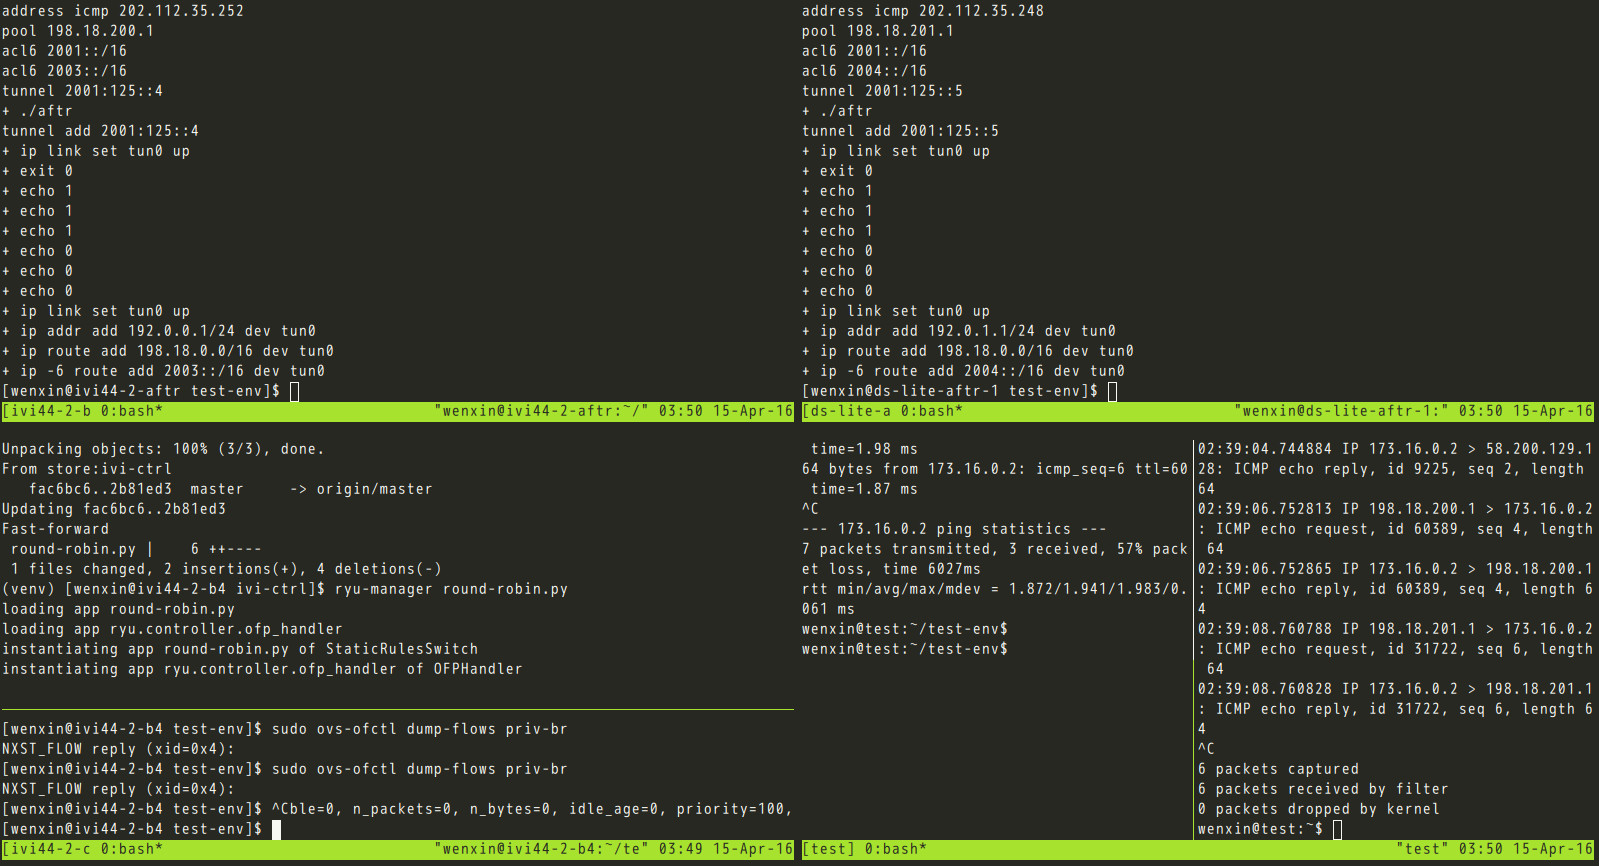
\includegraphics[width=\textwidth]{figs/test-env.jpeg}
  \end{center}
\end{frame}

\begin{frame}
  \frametitle{控制器}

  \begin{center}
    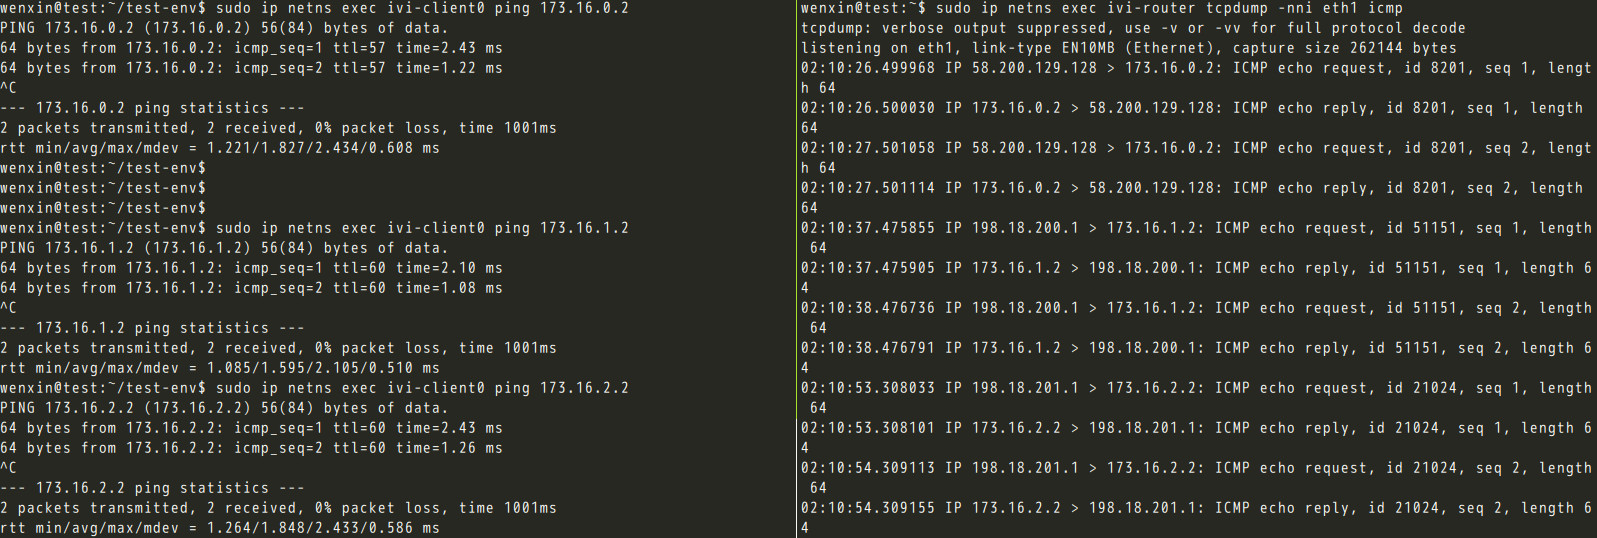
\includegraphics[width=\textwidth]{figs/static.jpeg}
  \end{center}

  \begin{center}
    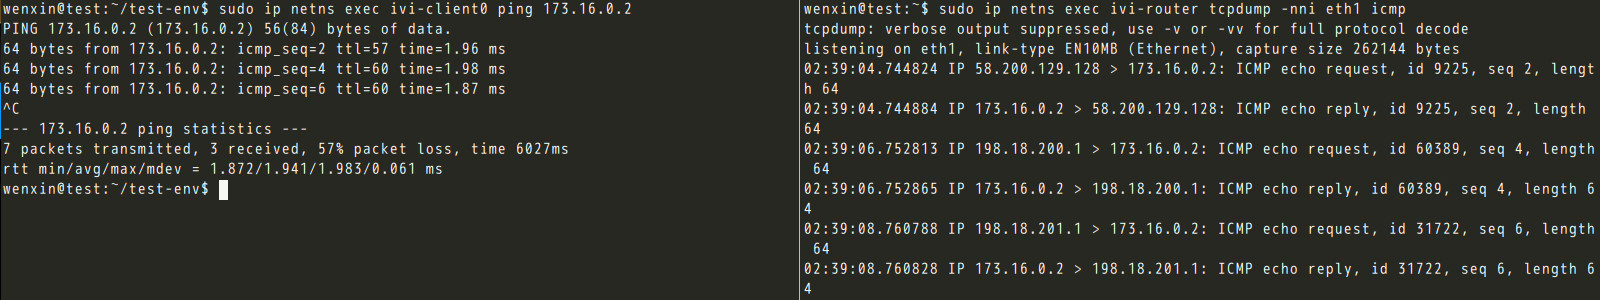
\includegraphics[width=\textwidth]{figs/round-robin.jpeg}  
  \end{center}
  
\end{frame}

\section{后续工作}
\begin{frame}
  \frametitle{后续工作}

  \begin{center}
    \includegraphics[width=0.8\textwidth]{figs/next-work.pdf}  
  \end{center}
  \begin{block}{}
    \begin{itemize}
    \item 在多个二级翻译器间控制调度
    \item 添加NAT64隧道
    \end{itemize}
  \end{block}
\end{frame}

\section{进度安排}

\begin{frame}
  \frametitle{进度安排}
  \begin{block}{}
    \begin{itemize}
    \item 4月15日-5月15日:实现多个翻译器间的调度
    \item 5月16日-答辩:封装接口,完善论文
    \end{itemize}
  \end{block}
\end{frame}

\section{参考文献}
\begin{frame}
  \frametitle{参考文献}
  \begin{itemize}
  \item \href{https://tools.ietf.org/html/rfc7599}{RFC7599}
  \item \href{https://tools.ietf.org/html/rfc7597}{RFC7597}
  \item \href{https://tools.ietf.org/html/rfc6219}{RFC6219}
  \item \href{https://tools.ietf.org/html/rfc6052}{RFC6052}
  \item \href{https://tools.ietf.org/html/rfc7598}{RFC7598}
  \item
    \href{http://openvswitch.org/}{Open vSwitch}
  \item
    \href{http://osrg.github.io/ryu/}{Ryu component-based software defined networking framework }
  \end{itemize}
\end{frame}

\section{Q\&A}

\begin{frame}
  \frametitle{Q\&A}
  \begin{center}
    {\LARGE 谢谢!}
    \vspace{3em}
    {\LARGE 请老师们提问和指导!}
  \end{center}
\end{frame}
\end{document}